\chapter{需求分析}
\label{chap:requirements}

\section{需求范围与功能总览}
本章依据当前源码梳理课程原型的身份、发现、通信、辅助、媒体及演示需求，编号用于报告追踪，验收条件不表示本次已执行测试。参与者为访客、已登录用户、相对角色“对方真人账号”、当前账号的演示操作者及外部文本、图片服务；AI 虚拟人物是内部设定，Demo 操作者不是管理所有账号的管理员。完整需求以项目需求文档及对应业务模块为准。

\begingroup
\songti\rmfamily\zihao{5}
\renewcommand{\arraystretch}{1.1}
\begin{longtable}{@{}p{.11\textwidth}p{.17\textwidth}p{.64\textwidth}@{}}
\caption{功能需求紧凑总览}\label{tab:requirements-summary}\\
\toprule 编号 & 功能 & 核心行为 \\
\midrule
\endfirsthead
\multicolumn{3}{c}{功能需求紧凑总览（续）}\\
\toprule 编号 & 功能 & 核心行为 \\
\midrule
\endhead
\midrule \multicolumn{3}{r}{续下页}\\
\endfoot
\bottomrule
\endlastfoot
FR-01 & 账号会话 & 注册、登录、退出；新登录替换旧会话，数据仍属原账号。 \\
FR-02 & 匹配资料 & 经同意提取标签；失败保留介绍并重试，期望介绍不公开。 \\
FR-03 & 相遇抽取 & 双向筛选、加权抽取；恢复待决定结果，不以刷新重抽。 \\
FR-04 & 收藏管理 & 喜欢、跳过、移除和冷却；移除不删历史交流。 \\
FR-05 & 真人纸条 & 收藏及接收资格校验，收件人接受并回信才建会话。 \\
FR-06 & 真人对话 & 双方本人发送、参与者权限校验、时间展示及轮询同步。 \\
FR-07 & 虚拟互动 & 明确标记模型回复；失败保留任务，重试不重发原消息。 \\
FR-08 & 拾言建议 & 切换风格、编辑建议或自行输入，明确点击才发送。 \\
FR-09 & 情绪展示 & 分析绑定最新对方消息，不可靠或缺图时回退默认立绘。 \\
FR-10 & 媒体管理 & 头像、背景、默认与各情绪立绘独立保存及删除。 \\
FR-11 & 情绪生图 & 另行授权参考图外发，后台任务、私有预览和版本确认。 \\
FR-12 & 感受授权 & 仅虚拟心笺、回望、揭晓及屏蔽；私人记录不发给模型。 \\
FR-13 & Demo 操作 & 注入预设来信、设虚拟意愿、推进日期及确认重置。 \\
FR-14 & 个人偏好 & 编辑本人展示名、习惯、话题及陌生人纸条接收开关。 \\
FR-15 & 交流参考 & 规则与可选模型组合，双方开关约束；在途撤回有缺口。 \\
\end{longtable}
\endgroup

\section{关键业务规则}
\begin{enumerate}[itemsep=2bp,topsep=3bp]
  \item 身份：用户名三至二十位字母、数字或下划线，密码八至一百二十八字符；会话固定三十天到期。注册两段介绍各十至五百字符并同意展示、分析，每组标签为固定词表中一至八个不重复项。
  \item 发现：任一方向标签无交集记零，否则取双向满足比例平均后的整数百分数；至少六十入池。排除本人、收藏、冷却对象；真人须开放接收且无会话或待回应纸条。金、紫、蓝对应九十五至一百、八十五至九十四、六十至八十四，不是成功概率。
  \item 收藏：五个位置初占三位虚拟“初始相遇”，不编匹配分数，移除不补回；先决定原抽取结果再抽，测试阶段每日不限次数，满员先移除。跳过、移除冷却三十天，不删除已有通信。
  \item 通信：纸条、首封回信一至一百字符，普通聊天一至五百；真人每日两张按服务器本地自然日计算，双方不能并存待回应纸条，接受回信与首轮消息事务提交。虚拟另有每日两次、待处理／暂存／归档防重复，日期受演示偏移影响。真人默认快照每会话最近五十条，无无限历史翻页。
  \item 辅助：三种解释、三项建议，四种风格为自然日常、轻松幽默、温柔关心、直接简短。真人约两秒轮询、隐藏暂停，另约六秒状态同步；对话分析绑定消息与风格，纸条草稿建议尚未复核迟到结果。真人可手动发送，虚拟待回复须先完成。真人情绪置信度至少七十且有图才切换立绘，否则默认图或问号人；虚拟人物使用固定内置立绘。
  \item 媒体与生图：PNG、JPEG、WebP；头像、立绘最多二百万字节，背景三百万。外发本人默认图须另行授权；每账号一个运行任务或待确认预览，全系统并发两次、每账号滚动二十四小时十二次，失败计次；超时一百八十秒、不自动重试，重启未完成任务标失败。状态查询或创建任务时清理超过七天的非运行记录，保存核对参考摘要和目标版本。
  \item 虚拟揭晓：初始化起每七天一周期，全周期一次而非每人物一次；须双向交流、本人当期积极意愿及授权、虚拟对方当期授权，资格不符不耗机会，跨期重授权，屏蔽停止互动并撤权。心笺零至一百分、备注最多二百字，不改变对方意愿。
  \item 真人参考：展示名最多二十字符，习惯、话题各一百；双方开关开启才查参考。模型有效时四因素各百分之二十五，否则节奏、连续性、文字占比为三十五、三十五、三十；缓存记末条消息编号与时间，非七天揭晓，也不确定真实好感。
\end{enumerate}
虚拟授权参数部分使用真值转换，非法类型可能误解；真人参考在模型请求开始校验双方开关，在途关闭仍可能返回旧分析。正常页面操作不等于严格授权或在途撤回保障。

\section{用例图与典型路径}
图\ref{fig:requirements-usecase}与图\ref{fig:requirements-usecase-ai}分离真人业务与虚拟／辅助业务。实线为参与关系，虚线箭头由可选行为指向基础用例（extend），或由基础用例指向必需行为（include）。登录只作前提，接受纸条只作建会话前置，不画成每次聊天都重复执行。

\begingroup
\tikzset{
  reqUC/.style={draw=ReportBlue,fill=ReportBlue!7,ellipse,align=center,text width=2.6cm,minimum height=.8cm,font=\small\linespread{1}\selectfont},
  reqActor/.style={align=center,text width=1.8cm,font=\small\linespread{1}\selectfont},
  reqRel/.style={dashed,-{Stealth[length=2mm]},draw=ReportTeal},
  reqLabel/.style={fill=white,inner sep=2pt,font=\footnotesize\linespread{1}\selectfont,align=center}}
\begin{figure}[htbp]
\centering
\resizebox{\textwidth}{!}{%
\begin{tikzpicture}[x=1cm,y=1cm]
  \draw[draw=ReportBlue,fill=ReportGray,rounded corners] (0,0) rectangle (10.5,7.4);
  \node[font=\small] at (5.25,7.1) {身份、发现与真人交流：系统边界};
  \node[reqActor] (visitor) at (-1.4,6.3) {访客};
  \node[reqActor] (user) at (-1.4,3.7) {已登录用户};
  \node[reqActor] (model) at (12,5) {外部文本模型};
  \node[reqActor] (other) at (12,2.4) {对方真人账号};
  \node[reqUC] (auth) at (2.8,6.3) {UC-01\\账号会话};
  \node[reqUC] (profile) at (2.8,5) {UC-02\\匹配资料};
  \node[reqUC] (draw) at (2.8,3.7) {UC-03\\抽取与收藏};
  \node[reqUC] (note) at (2.8,2.4) {UC-04\\递真人纸条};
  \node[reqUC] (chat) at (2.8,1.1) {UC-05\\回应与对话};
  \node[reqUC,fill=ReportTeal!7] (tags) at (8,5) {提取匹配标签};
  \node[reqUC,fill=ReportTeal!7] (score) at (8,1.1) {UC-14\\真人交流参考};
  \draw (visitor.east) -- (auth.west);
  \draw (user.east) -- (.35,3.7);
  \draw (.35,1.1) -- (.35,5.9) -- (auth.south west);
  \draw (.35,5) -- (profile.west);
  \draw (.35,3.7) -- (draw.west);
  \draw (.35,2.4) -- (note.west);
  \draw (.35,1.1) -- (chat.west);
  \draw (model.west) -- (tags.east);
  \draw (model.south) -- (11,4.2) -- (10.1,4.2) -- (10.1,1.1) -- (score.east);
  \draw (other.south) -- (11,.25) -- (2.8,.25) -- (chat.south);
  \draw[reqRel] (tags.west) -- node[reqLabel,above] {\texttt{<<extend>>}\\同意且请求分析} (profile.east);
  \draw[reqRel] (score.west) -- node[reqLabel,above] {\texttt{<<extend>>}\\双方开关开启} (chat.east);
\end{tikzpicture}}
\caption{身份、发现与真人交流用例图}
\label{fig:requirements-usecase}
\end{figure}

\begin{figure}[htbp]
\centering
\resizebox{\textwidth}{!}{%
\begin{tikzpicture}[x=1cm,y=1cm]
  \draw[draw=ReportBlue,fill=ReportGray,rounded corners] (0,0) rectangle (10.8,8.5);
  \node[font=\small] at (5.4,8.15) {虚拟互动、辅助与媒体：系统边界};
  \node[reqActor] (user) at (-1.4,4.6) {已登录用户};
  \node[reqActor] (operator) at (-1.4,.8) {演示操作者};
  \node[reqActor] (textai) at (12.2,6.5) {外部文本模型};
  \node[reqActor] (imageai) at (12.2,3.8) {外部图片服务};
  \node[reqUC] (virtual) at (2.8,7.1) {UC-06\\虚拟人物互动};
  \node[reqUC] (real) at (2.8,5.6) {UC-05\\真人对话入口};
  \node[reqUC] (media) at (2.8,3.8) {UC-09\\媒体管理};
  \node[reqUC] (feeling) at (2.8,2.3) {UC-11\\心笺与揭晓};
  \node[reqUC] (demo) at (2.8,.8) {UC-12\\设置与重置};
  \node[reqUC,fill=ReportTeal!7] (reply) at (8,7.1) {生成虚拟回复};
  \node[reqUC,fill=ReportTeal!7] (guide) at (8,5.6) {UC-07/08\\建议与情绪};
  \node[reqUC,fill=ReportTeal!7] (generate) at (8,3.8) {UC-10\\生图与确认};
  \node[reqUC] (pref) at (8,2.3) {UC-13\\个人偏好};
  \draw (user.east) -- (.35,4.6);
  \draw (.35,2.3) -- (.35,7.1);
  \draw (.35,7.1) -- (virtual.west);
  \draw (.35,5.6) -- (real.west);
  \draw (.35,3.8) -- (media.west);
  \draw (.35,2.3) -- (feeling.west);
  \draw (.35,2.3) -- (.8,2.3) -- (.8,.15) -- (8,.15) -- (pref.south);
  \draw (operator.east) -- (demo.west);
  \draw (textai.west) -- (10.4,6.5);
  \draw (10.4,5.6) -- (10.4,7.1);
  \draw (10.4,7.1) -- (reply.east);
  \draw (10.4,5.6) -- (guide.east);
  \draw (imageai.west) -- (generate.east);
  \draw[reqRel] (virtual.east) -- node[reqLabel,above] {\texttt{<<include>>}} (reply.west);
  \draw[reqRel] (guide.west) -- node[reqLabel,above] {\texttt{<<extend>>}\\选择 AI 辅助} (real.east);
  \draw[reqRel] (guide.north) -- (8,6.4) -- node[reqLabel,above] {\texttt{<<extend>>}} (2.8,6.4) -- (virtual.south);
  \draw[reqRel] (generate.west) -- node[reqLabel,above] {\texttt{<<extend>>}\\默认图及外发授权} (media.east);
\end{tikzpicture}}
\caption{虚拟互动、表达辅助与媒体用例图}
\label{fig:requirements-usecase-ai}
\end{figure}
\endgroup
第二幅图的 UC-05 是同一真人对话入口的重复展示，便于完整表示可选辅助关系，不是新用例。真人分析绑定最新对方消息，不替代本人发言；虚拟回复失败保留任务，标签提取和生图为条件扩展。

\textbf{发现与收藏（UC-01／02／03）。}账号及标签就绪后筛选、抽取，恢复原结果再决定；无候选、满员、未就绪须提示，移除保留历史。完整规约见表\ref{tab:requirements-uc-account}、表\ref{tab:requirements-uc-draw}。

\textbf{纸条与真人通信（UC-04／05）。}满足资格后投递，收件人接受回信才建会话；拒绝不建会话，非参与者不得读写，模型失败不阻止本人发言，见表\ref{tab:requirements-uc-real}。

\textbf{可选 AI 与媒体（UC-06 至 UC-14）。}建议只填草稿，过期或不可靠分析忽略、回退；生图授权、预览、版本确认后保存。虚拟授权与真人开关分别处理，见表\ref{tab:requirements-uc-ai}至表\ref{tab:requirements-uc-preferences}；总览见表\ref{tab:requirements-usecase-index}。

\section{原型入口与关键状态}
图\ref{fig:requirements-prototype-entry}及图\ref{fig:requirements-prototype-assistance}保留五张截图，以裁去外围背景及局部放大提高可读性，保持宽高比。取证于2026年11月4日1440$\times$1000视口、内存数据库及模拟模型，仅说明界面；来源见\texttt{assets/report/provenance.txt}。

\begin{figure}[htbp]
\centering
\begin{minipage}[c]{.29\textwidth}
  \centering
  
\includegraphics[width=\linewidth,keepaspectratio,trim=515bp 230bp 515bp 225bp,clip]{assets/report/login.png}
  \par\small （a）登录与注册入口
\end{minipage}\hfill
\begin{minipage}[c]{.68\textwidth}
  \centering
  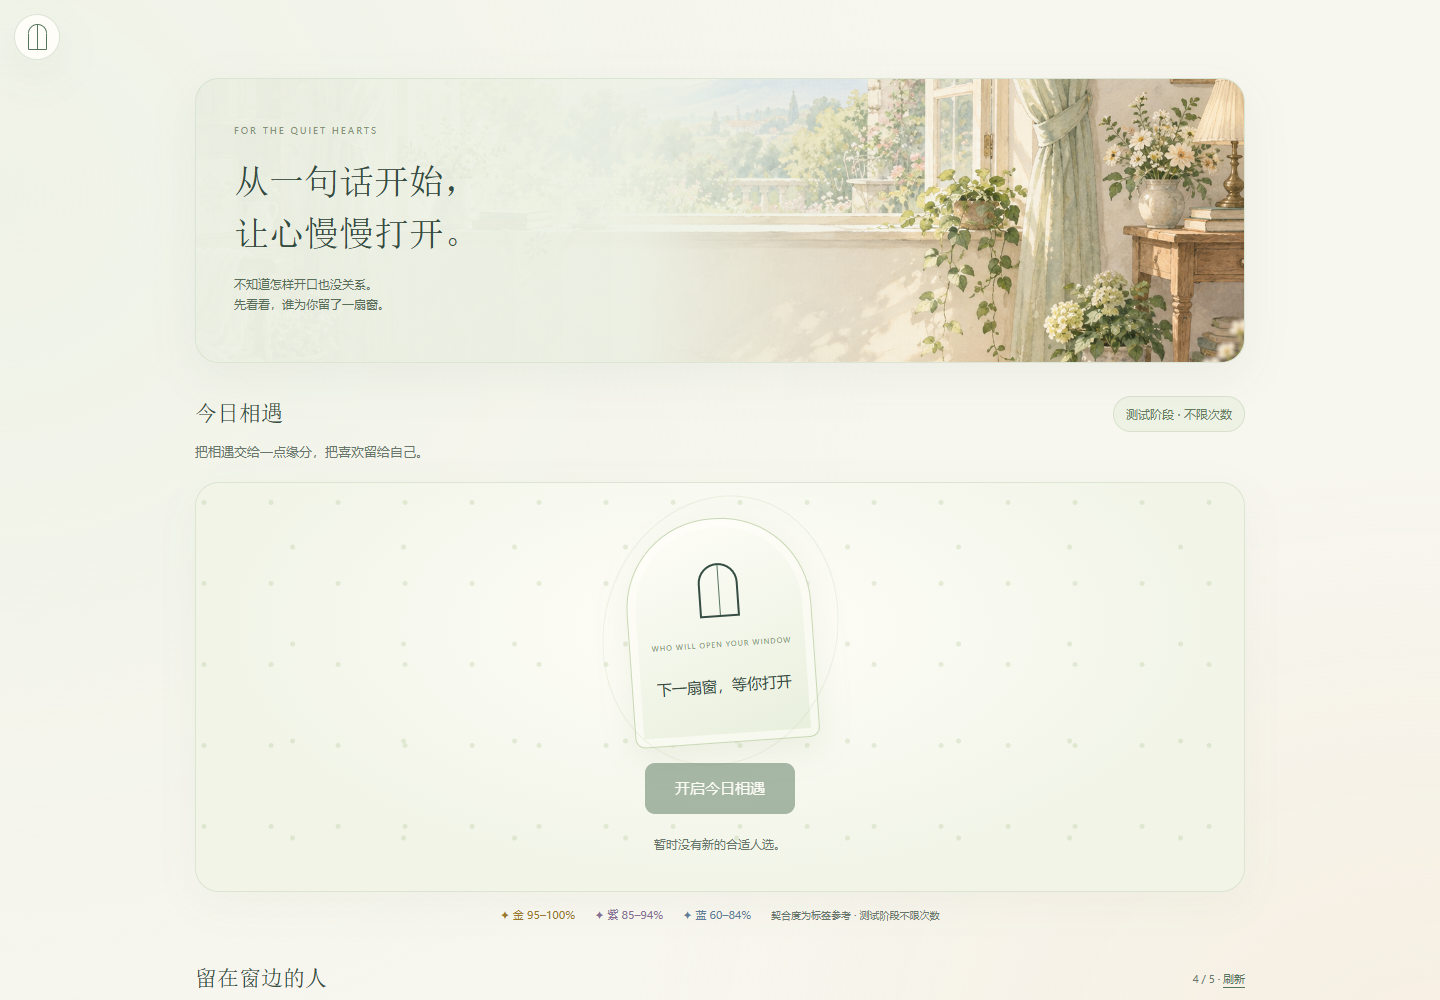
\includegraphics[width=\linewidth,keepaspectratio,trim=185bp 5bp 185bp 385bp,clip]{assets/report/meet.png}
  \par\small （b）遇见：无候选与收藏占位
\end{minipage}
\par\medskip
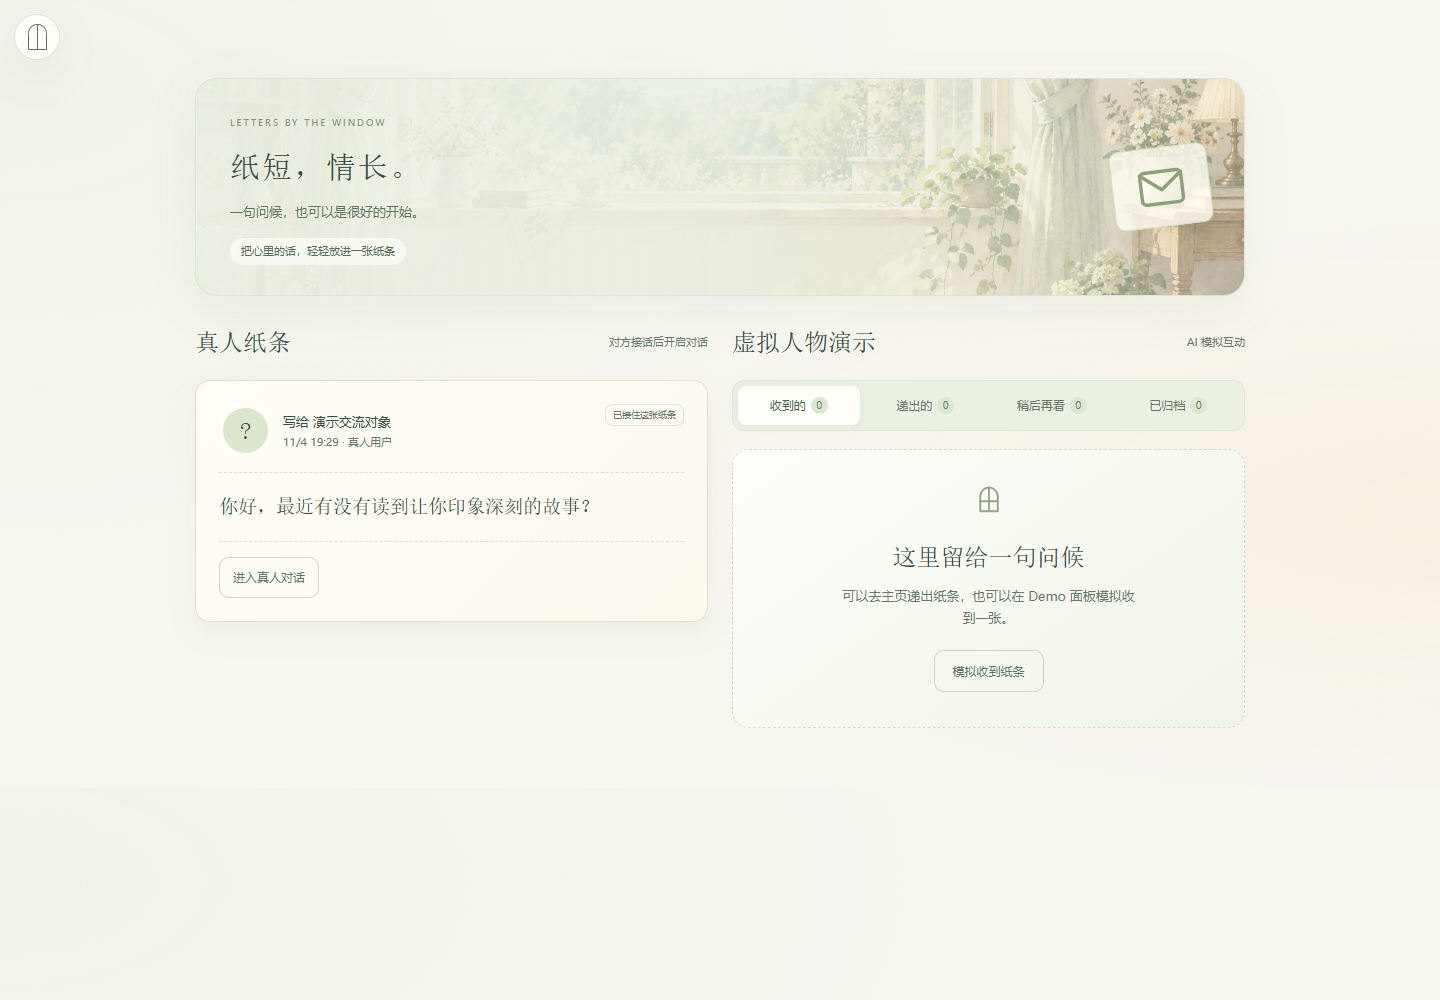
\includegraphics[width=.92\textwidth,keepaspectratio,trim=185bp 270bp 185bp 305bp,clip]{assets/report/notes.png}
\par\small （c）纸条：真人与虚拟入口分离
\caption{账号、发现与纸条原型图组（隔离演示，关键区域放大）}
\label{fig:requirements-prototype-entry}
\label{fig:requirements-login}
\label{fig:requirements-meet}
\label{fig:requirements-notes}
\end{figure}

账号入口收集凭据、介绍及同意；遇见区分身份、占位与无候选状态。纸条页按真人／虚拟类型和状态提供接受、拒绝、暂存或归档，回应只表示愿意交流。

\begin{figure}[htbp]
\centering
\begin{minipage}[c]{.35\textwidth}
  \centering
  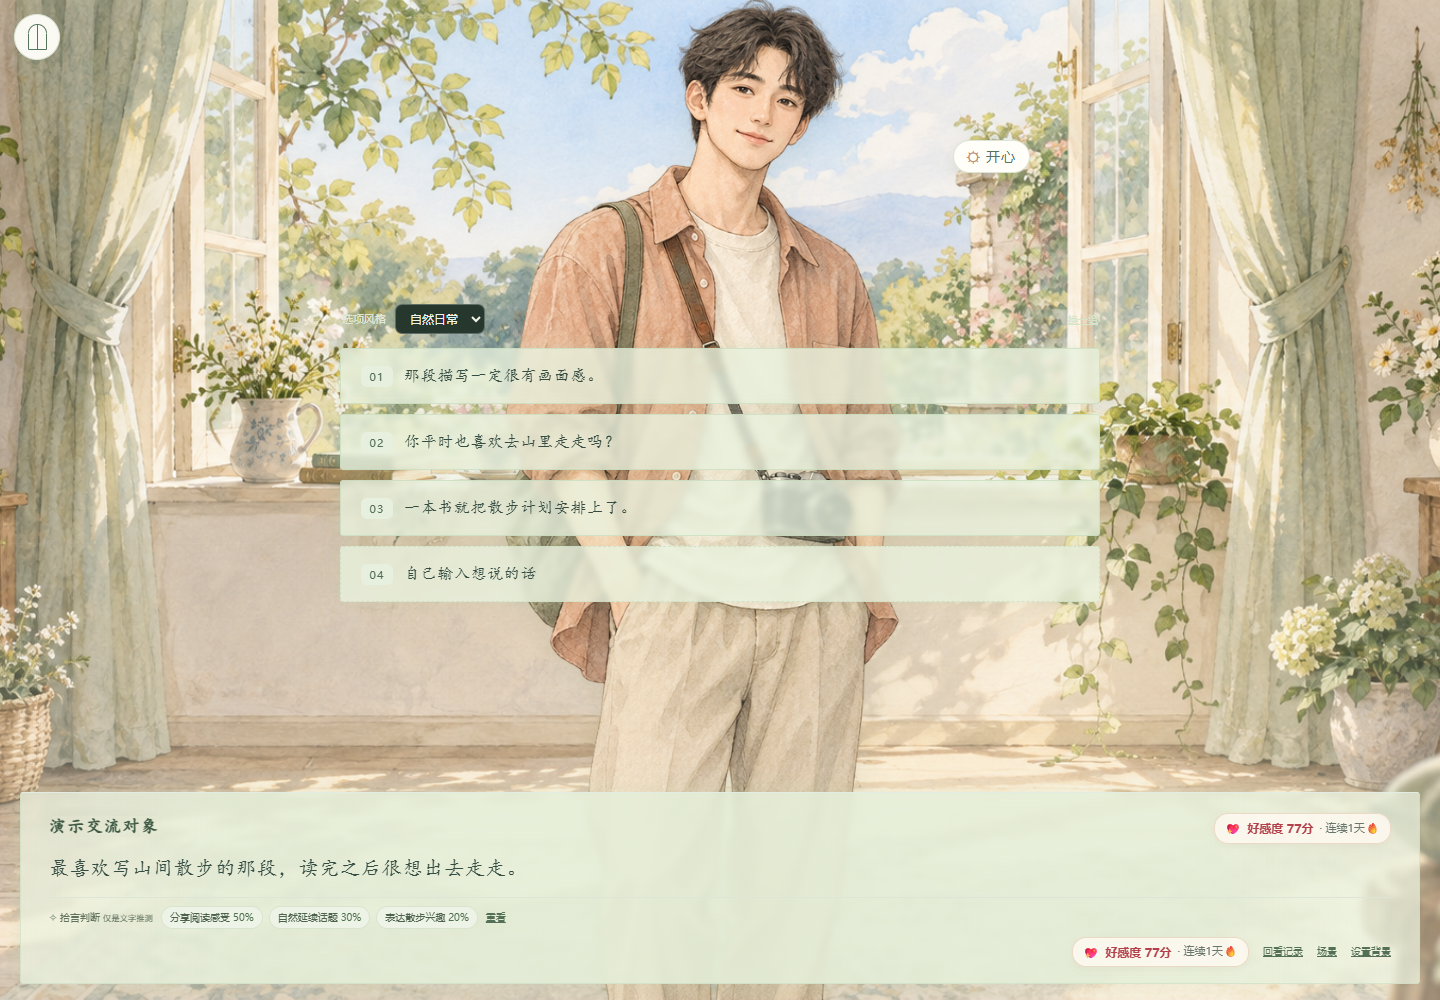
\includegraphics[width=\linewidth,keepaspectratio]{assets/report/chat.png}
  \par\small （a）对话整体布局
\end{minipage}\hfill
\begin{minipage}[c]{.62\textwidth}
  \centering
  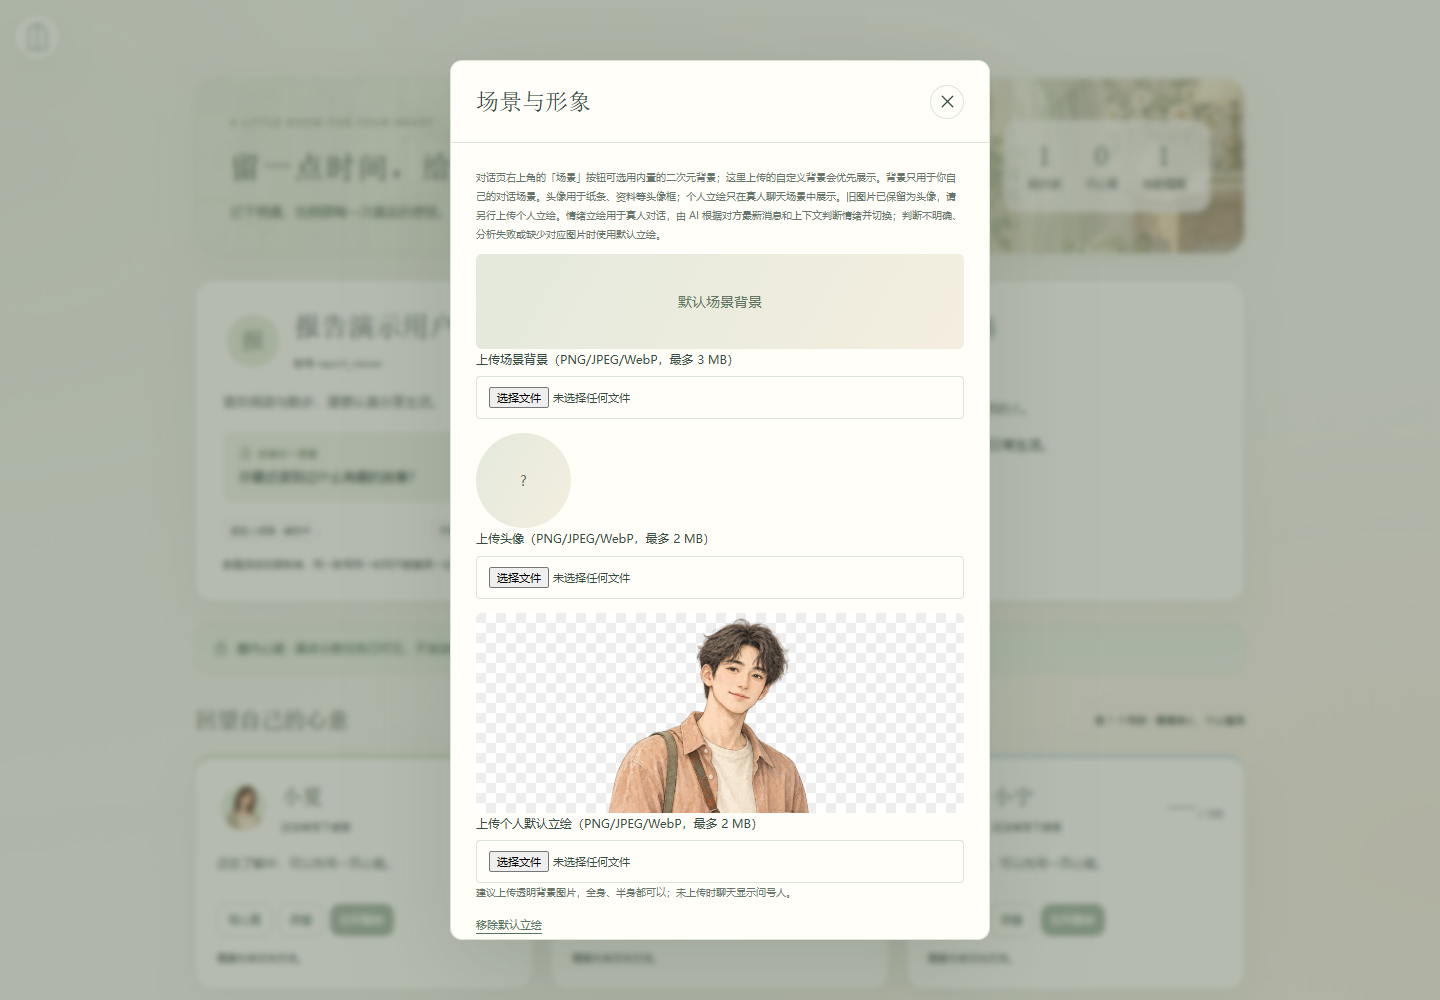
\includegraphics[width=\linewidth,keepaspectratio,trim=445bp 55bp 445bp 55bp,clip]{assets/report/media.png}
  \par\small （b）场景与形象设置
\end{minipage}
\par\medskip
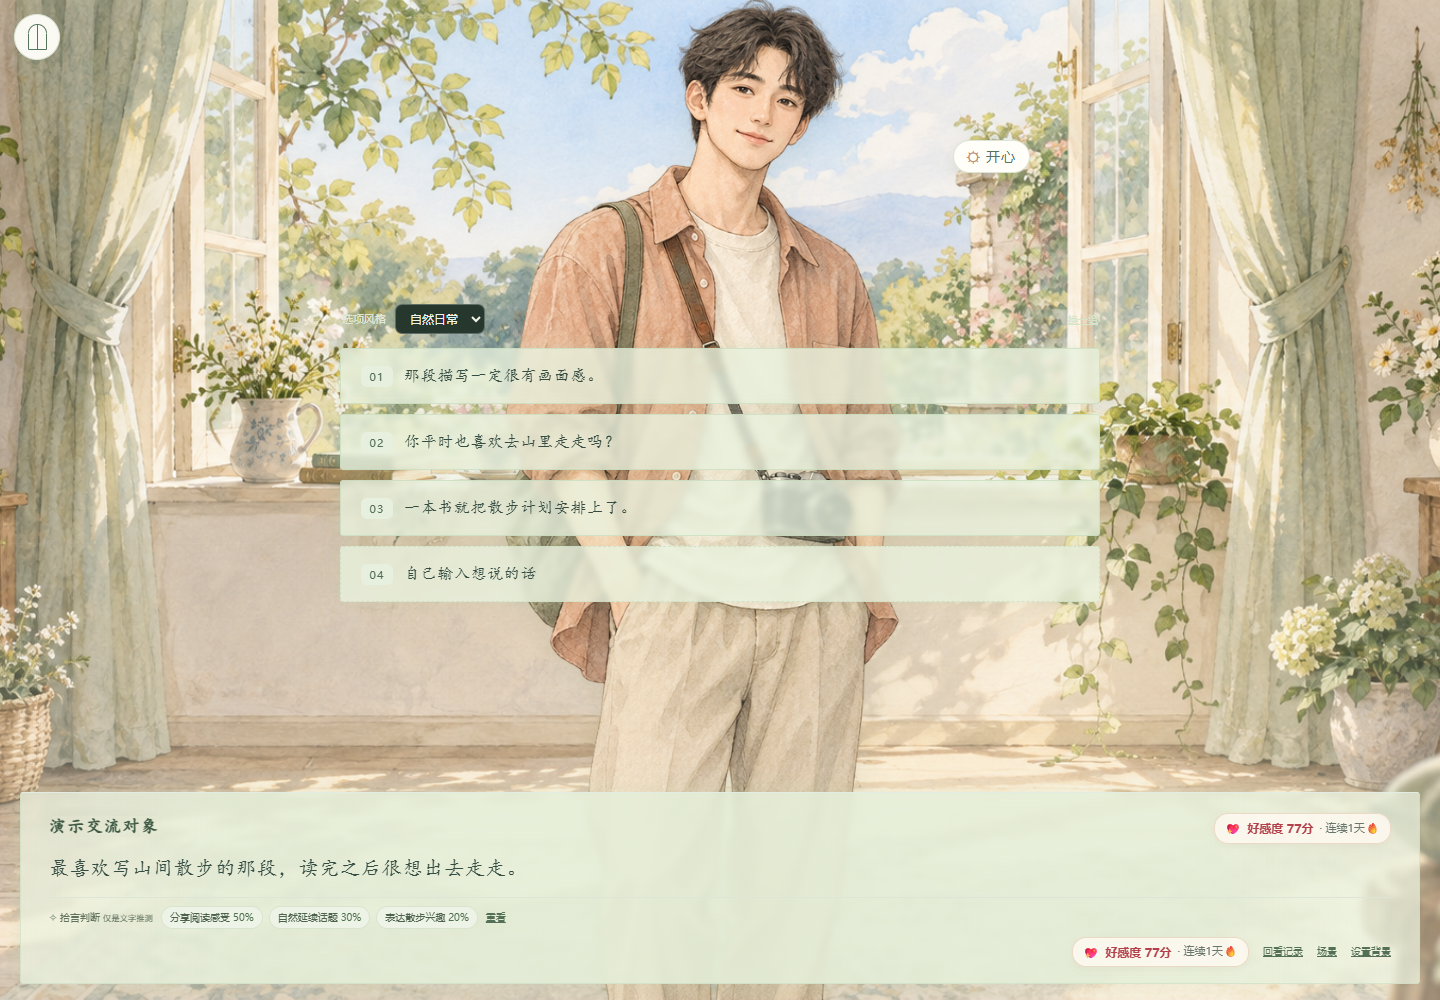
\includegraphics[width=\textwidth,keepaspectratio,trim=335bp 395bp 335bp 305bp,clip]{assets/report/chat.png}
\par\small （c）拾言建议局部放大：选择只填草稿，不自动发送
\caption{对话辅助与媒体原型图组（隔离演示）}
\label{fig:requirements-prototype-assistance}
\label{fig:requirements-chat}
\label{fig:requirements-media}
\end{figure}

对话展示时间、草稿和风格，情绪只绑定最新对方消息。媒体分别维护头像、背景和立绘，区分运行、失败、预览及已保存；真人参考开关不借用虚拟授权。

\section{非功能需求与验收边界}
详细机制与检查点见表\ref{tab:requirements-nonfunctional}。验收使用隔离账号、场景及模拟上游，检查成功、非法输入、越权和恢复，不操作日常数据或密钥；HTTP 与数据库未加密，真实身份、年龄、审核、无障碍、模型质量及生产保障须另行验证。

\begingroup
\songti\rmfamily\zihao{5}
\begin{longtable}{@{}p{.11\textwidth}p{.17\textwidth}p{.64\textwidth}@{}}
\caption{非功能需求摘要}\label{tab:requirements-nfr-summary}\\
\toprule 编号 & 质量属性 & 核心验收关注点 \\
\midrule
\endfirsthead
\multicolumn{3}{c}{非功能需求摘要（续）}\\
\toprule 编号 & 质量属性 & 核心验收关注点 \\
\midrule
\endhead
\midrule \multicolumn{3}{r}{续下页}\\
\endfoot
\bottomrule
\endlastfoot
NFR-01 & 访问安全 & 密码及令牌摘要、Cookie 防护、账号归属与会话参与者校验。 \\
NFR-02 & 数据最小化 & 凭据仅在服务端，核对模型载荷与参考图外发同意。 \\
NFR-03 & 可理解错误 & 中文业务错误与状态码，不泄露配置或上游原文。 \\
NFR-04 & 状态一致 & 事务与唯一约束，待决定复用、分析绑定及媒体版本检查。 \\
NFR-05 & 故障恢复 & 虚拟回复重试无重复，失效草稿尽力恢复，真人可手动通信。 \\
NFR-06 & 效率资源 & 快照及对话分析限量读消息，参考分读全量历史；并发与超时控制。 \\
\end{longtable}
\endgroup
